% Justificar la viabilidad del proyecto, indicando recursos humanos y tecnologicos, presupuesto inicial, etc, etc.

\section{Estudio de Viabilidad}

Para poder desarrollar este proyecto en su totalidad, deben tenerse en cuenta las consideraciones que se detallan a continuación.

\subsection{Recursos}
Es necesario tener en cuenta los recursos humanos, tecnológicos, y el coste económico asociado a la realización de este proyecto.

\subsubsection{Recursos Humanos}
Para poder realizar el proyecto son necesarios tres perfiles profesionales
\begin{itemize}
    \item 1 Desarrollador (responsable de la implementación del proyecto)
    \item 1 Ilustradora (responsable de la parte artística del proyecto)
    \item 2 Consultores (expertos en diferentes temas que se tratan en el proyecto y que orientaran en las diferentes tareas)
\end{itemize}
\textit{El equipo se verá más adelante en detalle en la Sección~\ref{sec:equipo} Equipo de Trabajo}.

\subsubsection{Recursos Tecnológicos}\label{sec:recurso-tecnologico}

Desde el punto de vista tecnológico para realizar el proyecto será necesario el computador con el que se realizará el desarrollo y el dispositivo móvil sobre el que correrá. Los detalles de estos dispositivos se presentan a continuación. 
\begin{table}[ht]
    \centering
    \begin{tabular}{|x|l|}
        \hline
        Tipo de dispositivo & Computador portátil \\
        \hline
        Sistema Operativo & Windows 10\\
        \hline
        Modelo & HP Envy 15\\
        \hline
        Procesador & Intel® i7-4712HQ\\
        \hline
    \end{tabular}
    \caption{Recurso: Laptop}
    \label{tab:pc}
\end{table}

\begin{table}[ht]
    \centering
    \begin{tabular}{|x|l|}
        \hline
        Tipo de dispositivo & Telefóno Móvil \\
        \hline
        Sistema Operativo & Android 9\\
        \hline
        Modelo & Huawei P20\\
        \hline
        Procesador & HiSilicon Kirin 970\\
        \hline
    \end{tabular}
    \caption{Recurso: Móvil}
    \label{tab:movil}
\end{table}


También será necesario disponer del siguiente software para un buen desarrollo del proyecto:
\begin{itemize}
    \item \textbf{\Gls{unity}:} \Gls{engine} utilizado para la creación del videojuego.
    \item \textbf{Visual Studio Community:} \gls{ide} utilizado para la programación de los scripts del videojuego. También fue utilizado para la edición de los documentos de texto relativos a la narrativa.
    \item \textbf{Paint Tool Sai:} Programa de ilustración digital.
    \item \textbf{Adobe Photoshop:} Programa de edición y creación de imágenes.
    \item \textbf{Audacity:} Programa de edición y grabación de audio.
\end{itemize}

La mayoría de los programas mencionados anteriormente son de uso gratuito (\Gls{unity}, Visual Studio, y Audacity). En el caso de los programas de paga los miembros del equipo que los usan ya contaban con una licencia adquirida previamente, por lo que no es necesaria una inversión monetaria inicial.


\subsubsection{Recursos Económicos}

El proyecto se planificó y desarrolló con un presupuesto monetario de 0 \euro{} y no se incurrieron en gastos adicionales para desarrollar el mismo. Sin embargo, no se descarta la necesidad de contar con un presupuesto monetario en caso de querer seguir trabajando e investigando más en un futuro.

\subsection{Investigaciones existentes}\label{sec:investigaciones}
Se realizó un estudio relativo a las investigaciones y juegos ya existentes que podían cubrir el mismo tema que planeaba investigar. 

Se utilizaron los buscadores \href{https://www.sciencedirect.com/}{Science Direct} y \href{https://www.springer.com/}{Springer} y se utilizaron las siguientes palabras claves: moral, videogames, moral dilemma, videogames and behaviour, videogames and feelings, influence of videogames.

Esta búsqueda arrojo aproximadamente 500 resultados distintos. Lluego para poder seleccionar el material se evaluó si tenían relación con alguno de estos tres conceptos: ``Moral en los videojuegos'', ``Influencias de los videojuegos en el comportamiento'', ``Decisiones de los jugadores''.

Estas investigaciones prueban que los videojuegos pueden influir en el comportamiento de las personas y sus emociones, ya sea afectando de forma positiva (Mejores habilidades cognitivas, beneficios motivacionales, emocionales o sociales) o negativa (generar ansiedad, agresividad, o comportamiento violento)\cite{impacts-games-behaviours}.

Asimismo se ha investigado respecto a los sistemas morales que implementan algunos juegos, y como fallan en ofrecer una empatía real con el jugador al ofrecer una perspectiva binaria y que carece de consecuencias reales para los jugadores\cite{ethics-single}\cite{only-game}. Aún así, mencionan que sin importar lo limitada que pueda ser aquella perspectiva, la decisión del jugador sigue siendo su responsabilidad  y no necesariamente es culpa del videojuego\cite{free-will}.

Un caso de uso que es relevante mencionar dentro de todas estas investigaciones es el de Papers Please, un juego que dentro de su simplicidad, aborda temas morales desde un punto de vista sistemático en lugar de un punto de vista pre-escrito. Esto quiere decir que en lugar de tener una narrativa que se divide y se presenta como conversación, Papers Please maneja la moral como un elemento del juego que el jugador debe interpretar\cite{papers}.

Para este proyecto se decidió utilizar el punto de vista pre-escrito, ya que ofrece mayor control respecto a lo que interpreta el jugador y esto nos ayuda a tratar de influenciar al jugador, que es uno de los objetivos de esta investigación.


%\textbf{Como hiciste la busqueda?? Biscadores, palabras clave y criterios de selección.
%3 juegos es muy poco. Me parece bien que solo expliques estos tres però tienes que hacer la busqueda videogames and feelings, Influences of videogames in players
%The Impact of Video Games on the Players Behaviors: A Survey Hay bastante literatura al respecto. Debes hacer referencia a ella !!}


%La moralidad es un tópico recurrente dentro de los videojuegos, así como los dilemas morales que éstos pueden presentar, debido a ello las investigaciones relativas a la moral no son del todo nuevas, sin embargo lo que ellas hacen es simplemente un análisis del mismo.

%En "The Ethics of Choice in Single-Player Video Games" \cite{ethics-single} la investigación se enfoca en los daños o beneficios que un videojuego puede causar en las personas, particularmente en el caso de los juegos de un solo jugador, y como las decisiones que toman -o las que asume la historia- los puede influir. Como ejemplos considérense los juegos siguientes.

%En "It's only a game" \cite{only-game} se analiza como los juegos tienden a adoptar una perspectiva binaria y utilitaria, así como también fallan en ofrecer una empatía real con el jugador -de manera tal que se refleje su moral-. Hace una revisión también en la narrativa y en los tópicos de la moral y la ética que se ha utilizado en los videojuegos.

%Por otro lado, está "The Influence of Empathy and Morality of Violent Video Game Characters on Gamers' Aggresion" \cite{violent-gamer} donde se estudía la influencia que pueden tener los personajes en los jugadores. Principalmente, se considera como el empatizar con estos personajes y con su moral, afecta en la influencia que puedan tener en las personas.

%Estás 3 investigaciones abordan la moral en los videojuegos y cada una se enfoca en un aspecto en particular y distinto del que se abarcará en este proyecto. Dado que este proyecto lo que busca es analizar experimentalmente si un videojuego puede influir y hacer cambiar de opinión a un jugador (o no). \textbf{En los que has mencionado no hay estudio experimental?? Asegurate de que es así}



Por el lado de los videojuegos existentes hay dos juegos en particular donde la moral del jugador es parte importante del videojuego: \textbf{Undertale} (2015) y \textbf{Detroit: Become Human} (2018). Ambos juegos comparten una característica crucial que es ``Tus decisiones importan''. Los diálogos, las escenas y los eventos que ves (o no) en el juego se determinan en base a las acciones que has realizado previamente. En Undertale el efecto es menos obvio o inmediato y hay algunos detalles que no sueles darte cuenta hasta más adelante en el juego, mientras que por otro lado en Detroit: Become Human, el juego te muestra todas las bifurcaciones posibles de la historia al termino de cada capitulo, y te ofrece la oportunidad de volver a un punto en específico en caso que desees experimentar una nueva opción o te arrepientas de las decisiones que tomaste.

\begin{figure}
    \centering
    \begin{minipage}{.49\textwidth}
        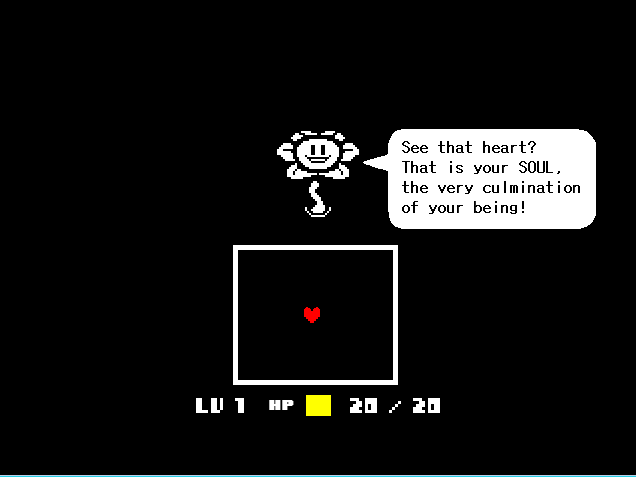
\includegraphics[width=\textwidth]{imgs/undertale.png}
        \caption{Undertale}
        \label{fig:undertale}
    \end{minipage}
    \begin{minipage}{.49\textwidth}
        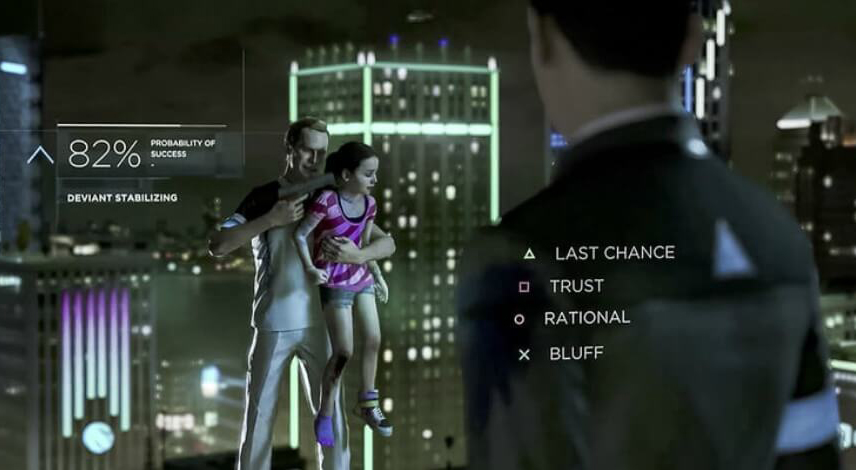
\includegraphics[width=\textwidth]{imgs/detroit-choices.jpg}
        \caption{Detroit: Became Human}
        \label{fig:detroit}
    \end{minipage}
\end{figure}

La mayor diferencia que poseen estos juegos con mi investigación, es que estos juegos solo hacen que el jugador se vuelva consciente de su moral y las decisiones que toma -y las pueda cuestionar o empatizar más con el juego-, pero no lo busca hacer cambiar de opinión ni trata deliberadamente de influir en el jugador, que es el eje principal de este proyecto.

\subsection{Público Objetivo}

El videojuego que se desarrollará en esta investigación, está dirigido a un público de entre 17 a 24 años. Adolescente - Adulto Joven que asiste a la Educación Superior o está por egresar de esta. De clase media-media baja y que posee un \gls{smartphone}.